\documentclass{article}
\usepackage[utf8]{inputenc}
\usepackage[T1]{fontenc}
\usepackage[french]{babel}
\usepackage{graphicx}

\title{Rendu n.2 Projet technologique}
\author{Zoé Debaty}
\date{Janvier 2020}

\begin{document}

\maketitle
\tableofcontents 
\newpage

% --------- Specificites techniques --------- %
\section{Spécificités techniques}

% --- L'image --- %
\subsection{Les images}
\subsubsection{Multicolor}
\begin{center} 
    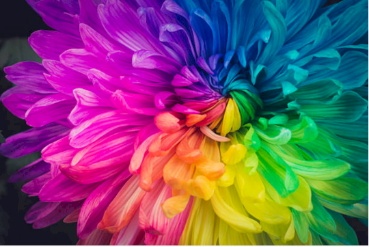
\includegraphics[width=9cm]{../Image_fonctions/Multicolor/Base.PNG}
\end{center}
\bigbreak

\begin{itemize}
\item Nom : "multicolor"
\item Dimensions : 612p * 408p
\item Taille : 59,9 Ko
\end{itemize}
\medbreak

L'image a été choisie car elle possède des changements de luminosité et énormément de couleurs afin de tester au mieux mes fonctions.

\subsubsection{Cat}
\begin{center} 
    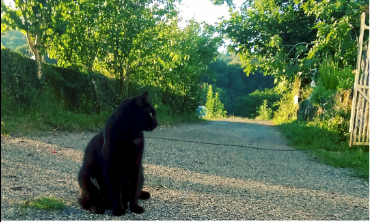
\includegraphics[width=9cm]{../Image_fonctions/Cat/Base.PNG}
\end{center}
\bigbreak

\begin{itemize}
\item Nom : "cat"
\item Dimensions : 1728p * 1036p
\item Taille : 1,87 Mo
\end{itemize}
\medbreak

Cette image est très grande et lourde et me permet de tester mes fonctions dans des cas extrêmes.

\subsubsection{Girl}
\begin{center} 
    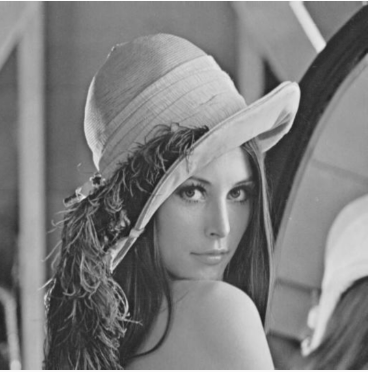
\includegraphics[width=9cm]{../Image_fonctions/Lenna/Base.PNG}
\end{center}
\bigbreak

\begin{itemize}
\item Nom : "Girl"
\item Dimensions : 512p * 512p
\item Taille : 31,4 Ko
\end{itemize}
\medbreak

Cette image est la plus légère et petite. Elle est de base en noir et blanc et est souvent utilisée en exemple dans les cours.
Elle me permet de tester facilement des fonctions de convolution.

% --- Le telephone --- %
\subsection{Le téléphone}
Pour tester mes fonctions j'utilise un Sony Xperia XA, avec un écran de 5 pouces.
Il tourne sous Android Nougat 7.0.

Toutes les performances ont été calculées sur ce téléphone. 
Les images ont été prises sur un émulateur Pixel 2 tournant sous Android 7.0.
\newpage

% ---------------- L'interface ---------------- %

\section{Interface}

% --- Page principale --- %
\subsection{Page principale}
La page d'accueil de mon application de sépare en trois parties. 

\begin{center} 
    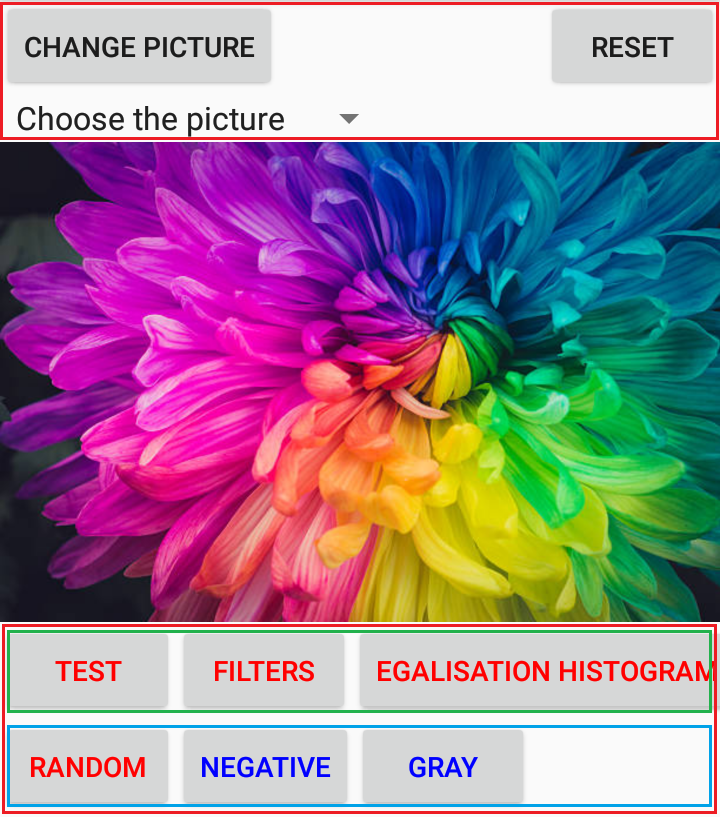
\includegraphics[width=9cm]{../Screen.png}
\end{center}

\begin{itemize}
    \item Au centre de l'écran se trouve l'image courante.
    \item Au dessus de l'image, le bouton « reset » reviendra à l'image de base (à noter que si on se trouve dans la partie convolution, l'image de base sera grisée) et le bouton « change picture » appliquera l'image choisie dans le menu déroulant dessous (voir nom d'images ci dessus).
    \item Au dessous de l'image se trouve deux menu horizontaux. La partie du haut (rectangle vert) correspond aux fonctions écrites en langage JAVA. La partie du dessous (rectangle bleu) correspond aux fonctions écrites en langage RenderScript.
    Un bouton écrit en bleu représente une fonctions RenderScript fonctionnelle. 
    Un bouton écrit en rouge représente une fonction non fonctionnelle.
    Le bouton test me permet de tester rapidement de nouvelles fonctions.
\end{itemize}

% --- Pages secondaires --- %
\subsection{Pages secondaires}
\medbreak
Pour les fonctions modifiant la saturation et la luminosité, un sous menu apparaîtra pour choisir à ajouter ou enlever la saturation/luminosité.

Pour la sélection de couleur, j'ai utilisé quatre boutons afin d'ajouter ou d'enlever des couleurs à gauche ou a droite de 0 (sur un cercle de 0 à 360). 

Le bouton "filters" accède à un nouveau menu défilant horizontalement permettant de choisir parmi les différents filtres de convolutions implémentés. D'autres boutons afin de choisir la taille du filtres pourront apparaître en fonction du filtre choisi.
\bigbreak

% --- Integration --- %
\subsection{Integration}
Je me suis aussi rendue compte que mon application ne s’adaptait pas aux barres de navigation virtuelles (contrairement aux téléphones possédant des boutons physique). En effet, certains boutons étaient cachés par la barre. 
J'ai donc résolu ce problème en modifiant la visibilité de l'interface utilisateur au lancement de l'application. Mais quelques problèmes sont encore à gérer (voir Bugs).

\newpage

% ---------------- Fonctions ---------------- %
\section{Fonctions}

\subsection{TD 1 Introduction}
% --- Gris ---%
\subsubsection{Griser l'image}

Cette fonction passe une image RGB en teintes de gris.

\begin{center} 
    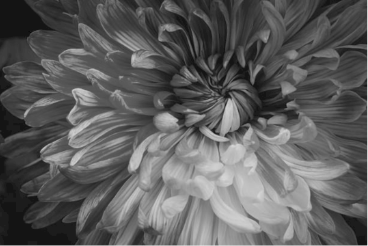
\includegraphics[width=9cm]{../Image_fonctions/Multicolor/Gray.PNG}
\end{center}
\begin{center} 
    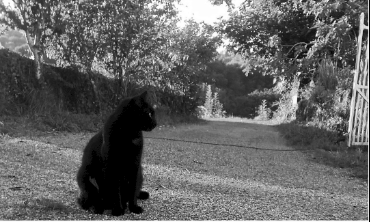
\includegraphics[width=9cm]{../Image_fonctions/Cat/Gray.PNG}
\end{center}
\begin{center} 
    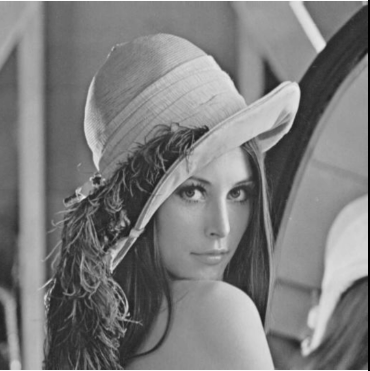
\includegraphics[width=9cm]{../Image_fonctions/Lenna/Gray.PNG}
\end{center}

\begin{center}
\medbreak
Test de performance de la fonction en microsecondes
\bigbreak
   \begin{tabular}{ | l | c | }
     \hline
     Image & Temps \\
     \hline
     Multicolor & 137 074 \\
     \hline
     Cat & 655 171 \\
     \hline
     Girl & 75 024 \\
     \hline
   \end{tabular}
 \end{center}
 \bigbreak

\newpage
\subsection{TD 2 Profilage de couleur}

% --- Coloriser --- %
\subsubsection{Coloriser l'image}

Cette fonction colore une image RGB avec une couleur aléatoire.

\begin{center} 
    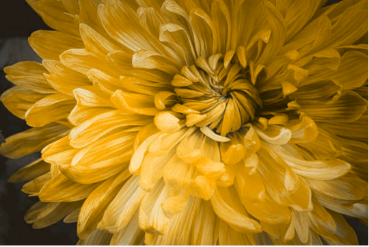
\includegraphics[width=9cm]{../Image_fonctions/Multicolor/Random.PNG}
\end{center}
\begin{center} 
    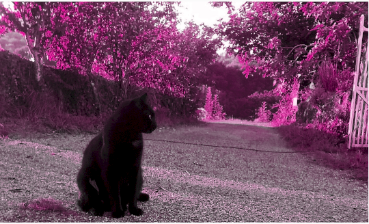
\includegraphics[width=9cm]{../Image_fonctions/Cat/Random.PNG}
\end{center}
\begin{center} 
    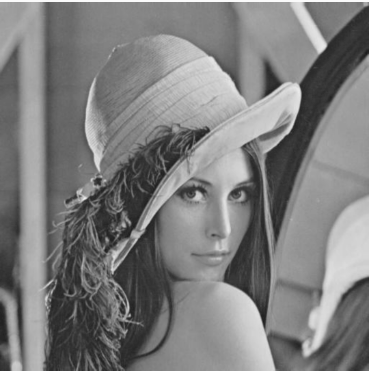
\includegraphics[width=9cm]{../Image_fonctions/Lenna/Random.PNG}
\end{center}

\begin{center}
\medbreak
Test de performance de la fonction en microsecondes
\bigbreak
   \begin{tabular}{ | l | c | }
     \hline
     Image & Temps \\
     \hline
     Multicolor & 754 872 \\
     \hline
     Cat & 5 368 410 \\
     \hline
     Girl & 755 697 \\
     \hline
   \end{tabular}
 \end{center}
\bigbreak

% --- HSVtoRGB --- %
\subsubsection{HSVtoRGB et inversement}

Afin de tester mes fonctions HSVtoRGB et RGBtoHSV, j'ai fait en sorte de les appeler à la suite (l'image ne change donc pas) et je compare la performance à celle des fonctions de bases dans le package Color.

\begin{center}
\medbreak
Test de performance du passage de RGB en HSV et inversement en microsecondes
\bigbreak
   \begin{tabular}{ | l | c | c |}
     \hline
     Image & Temps fonctions de bases & Temps fonctions réécrites \\
     \hline
     Multicolor & 11 080 625 & 927 161\\
     \hline
     Cat & > 1 min & 5 410 279 \\
     \hline
     Girl & 11 423 849 & 818 137 \\
     \hline
   \end{tabular}
 \end{center}
\bigbreak

% --- Garder une couleur --- %
\subsubsection{Garder une couleur}

Cette fonction permet, au moyen de deux limites que l'on modifies de 10 en 10, de garder seulement certaines couleurs sur l'image. La fonction se basant sur la couleur de l'image, elle ne sera pas testée sur l'image "Girl".

\begin{center} 
    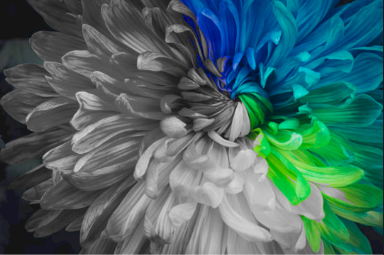
\includegraphics[width=9cm]{../Image_fonctions/Multicolor/SelectedColor.PNG}
    
    Exemple d'utilisation de la fonction sur Multicolor afin de ne garder que les parties bleues et vertes.
    
    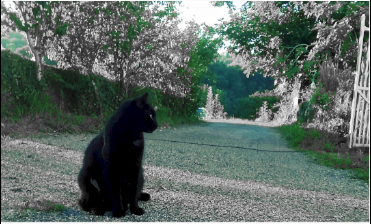
\includegraphics[width=9cm]{../Image_fonctions/Cat/SelectedColor.PNG}
    
    Exemple d'utilisation de la fonction sur Cat afin de ne garder que les parties vertes.
\end{center}
\bigbreak

% +10 Droite %
\textbf{-> +10 Droite}

\begin{center} 
    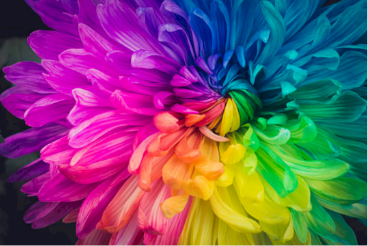
\includegraphics[width=9cm]{../Image_fonctions/Multicolor/Selected+10R.PNG}
\end{center}
\begin{center} 
    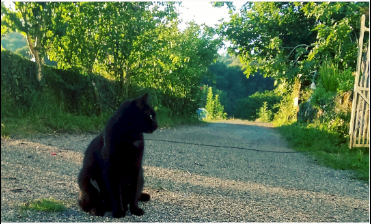
\includegraphics[width=9cm]{../Image_fonctions/Cat/Selected+10R.PNG}
\end{center}

\begin{center}
\medbreak
Test de performance de la fonction en appliquant + 10 Droite en microsecondes
\bigbreak
   \begin{tabular}{ | l | c | }
     \hline
     Image & Temps \\
     \hline
     Multicolor & 744 703 \\
     \hline
     Cat & 5 675 636 \\
     \hline
   \end{tabular}
 \end{center}

\bigbreak

% -10 Droite %
\textbf{-> -10 Droite}

\begin{center} 
    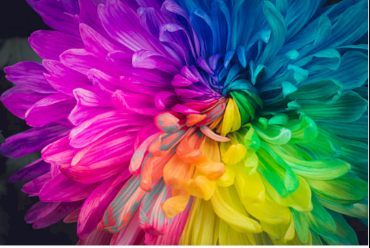
\includegraphics[width=9cm]{../Image_fonctions/Multicolor/Selected-10R.PNG}
\end{center}
\begin{center} 
    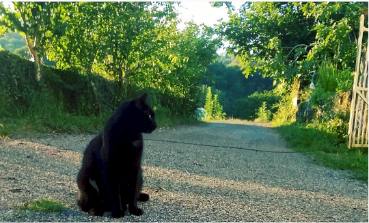
\includegraphics[width=9cm]{../Image_fonctions/Cat/Selected-10R.PNG}
\end{center}

\begin{center}
\medbreak
Test de performance de la fonction en appliquant - 10 Droite en microsecondes
\bigbreak
   \begin{tabular}{ | l | c | }
     \hline
     Image & Temps \\
     \hline
     Multicolor & 738 497 \\
     \hline
     Cat & 5 222 368 \\
     \hline
   \end{tabular}
 \end{center}
 
\bigbreak

% +10 Gauche %
\textbf{-> +10 Gauche}

\begin{center} 
    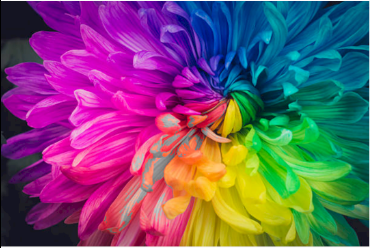
\includegraphics[width=9cm]{../Image_fonctions/Multicolor/Selected+10L.PNG}
\end{center}
\begin{center} 
    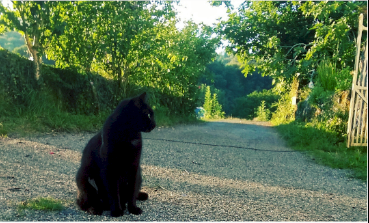
\includegraphics[width=9cm]{../Image_fonctions/Cat/Selected+10L.PNG}
\end{center}

\begin{center}
\medbreak
Test de performance de la fonction en appliquant + 10 Gauche en microsecondes
\bigbreak
   \begin{tabular}{ | l | c | }
     \hline
     Image & Temps \\
     \hline
     Multicolor & 746 670 \\
     \hline
     Cat & 5 377 165 \\
     \hline
   \end{tabular}
 \end{center}
 
\bigbreak

% -10 Gauche %
\textbf{-> -10 Gauche}

\begin{center} 
    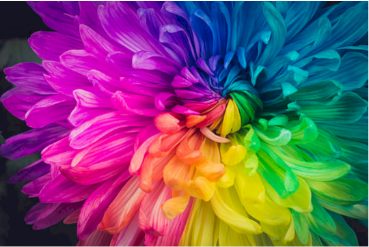
\includegraphics[width=9cm]{../Image_fonctions/Multicolor/Selected-10L.PNG}
\end{center}
\begin{center} 
    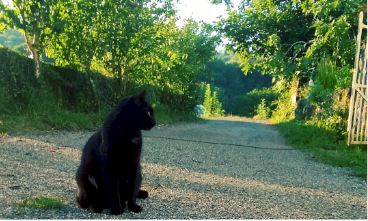
\includegraphics[width=9cm]{../Image_fonctions/Cat/Selected-10L.PNG}
\end{center}

\begin{center}
\medbreak
Test de performance de la fonction en appliquant - 10 Gauche en microsecondes
\bigbreak
   \begin{tabular}{ | l | c | }
     \hline
     Image & Temps \\
     \hline
     Multicolor & 714 794 \\
     \hline
     Cat & 5 510 806 \\
     \hline
   \end{tabular}
 \end{center}
 
 \bigbreak
 
 % Remarques %
 \textbf{ -> Remarques}
 On peut voir qu'il n'y a pas de changement pour l'image "Cat" dans les tests de +10 et -10, en effet, les limites sont placées à 0 et 360 au lancement du programme. Cette marge correspond au rouge et ,n'ayant pas de rouge dans cette image, on n'y voit pas de différence.

\newpage
\subsection{TD 3 Contraste et Histogrammes}
% --- Extension Gray --- %
\subsubsection{Extension de dynamique sur image grise}

Cette fonction
 applique une extension de dynamique sur une image en teintes de gris.

\begin{center} 
    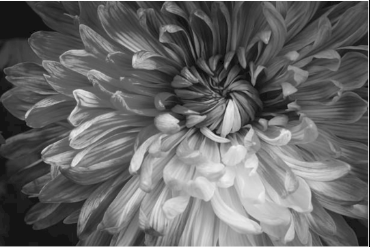
\includegraphics[width=9cm]{../Image_fonctions/Multicolor/LinearGray.PNG}
\end{center}
\begin{center} 
    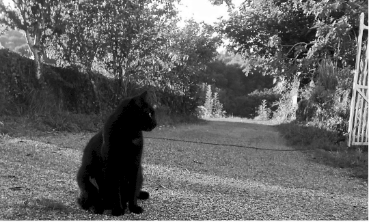
\includegraphics[width=9cm]{../Image_fonctions/Cat/LinearGray.PNG}
\end{center}
\begin{center} 
    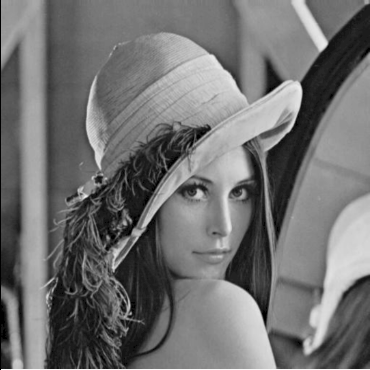
\includegraphics[width=9cm]{../Image_fonctions/Lenna/LinearGray.PNG}
\end{center}

\begin{center}
\medbreak
Test de performance de la fonction sur une image en teinte de gris en microsecondes
\bigbreak
   \begin{tabular}{ | l | c | }
     \hline
     Image & Temps \\
     \hline
     Multicolor & 96 935 \\
     \hline
     Cat & 748 597 \\
     \hline
     Girl & 121 769 \\
     \hline
   \end{tabular}
 \end{center}
 \bigbreak

% --- Extension Color --- %
\subsubsection{Extension de dynamique sur image couleur}

Cette fonction applique une extension de dynamique sur une image en couleur. La fonction se basant sur la couleur de l'image, elle ne sera pas testée sur l'image "Girl".

\begin{center} 
    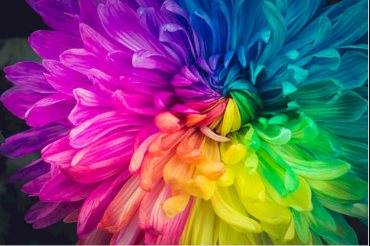
\includegraphics[width=9cm]{../Image_fonctions/Multicolor/LinearColor.PNG}
\end{center}
\begin{center} 
    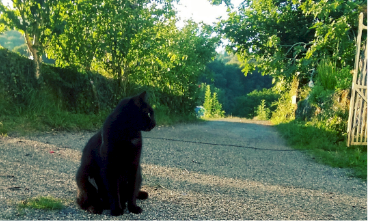
\includegraphics[width=9cm]{../Image_fonctions/Cat/LinearColor.PNG}
\end{center}

\begin{center}
\medbreak
Test de performance de la fonction sur une image en couleur en microsecondes
\bigbreak
   \begin{tabular}{ | l | c | }
     \hline
     Image & Temps \\
     \hline
     Multicolor & 145 012 \\
     \hline
     Cat & 561 235 \\
     \hline
   \end{tabular}
 \end{center}
\bigbreak

% --- Egalisation Gray --- %
\subsubsection{Égalisation d'histogramme sur image grise}

Cette fonction applique une égalisation d'histogramme sur une image en teintes de gris.

\begin{center} 
    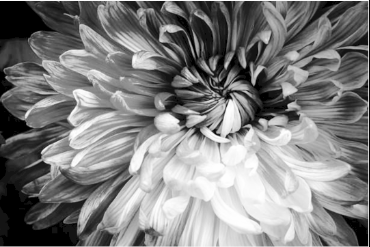
\includegraphics[width=9cm]{../Image_fonctions/Multicolor/EgalisationGray.PNG}
\end{center}
\begin{center} 
    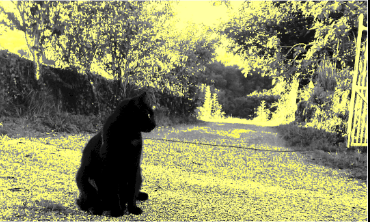
\includegraphics[width=9cm]{../Image_fonctions/Cat/EgalisationGray.PNG}
    
    (Image prise sur l'émulateur)
    
    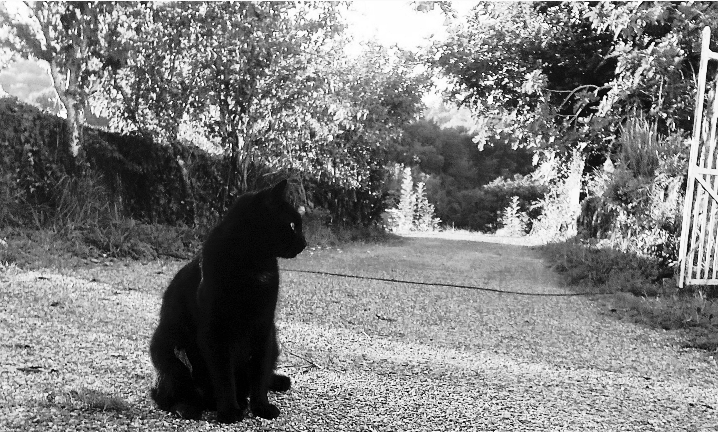
\includegraphics[width=9cm]{../Image_fonctions/Cat/EgalisationGray2.PNG}
    
    (Image prise sur le Sony)
\end{center}
\begin{center} 
    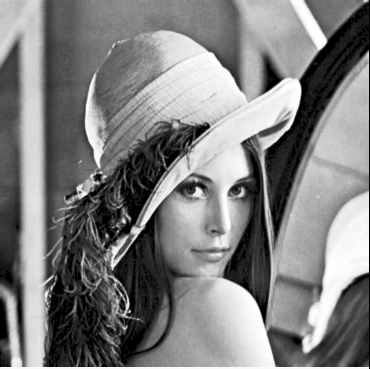
\includegraphics[width=9cm]{../Image_fonctions/Lenna/EgalisationGray.PNG}
\end{center}

\begin{center}
\medbreak
Test de performance de la fonction sur une image en teintes de gris en microsecondes
\bigbreak
   \begin{tabular}{ | l | c | }
     \hline
     Image & Temps \\
     \hline
     Multicolor & 270 230 \\
     \hline
     Cat & 1 021 697 \\
     \hline
     Girl & 288 203 \\
     \hline
   \end{tabular}
 \end{center}
\bigbreak

% --- Egalisation Color --- %
\subsubsection{Égalisation d'histogramme sur image couleur}

Cette fonction applique une égalisation d'histogramme sur une image en couleur. La fonction se basant sur la couleur de l'image, elle ne sera pas testée sur l'image "Girl".

\begin{center} 
    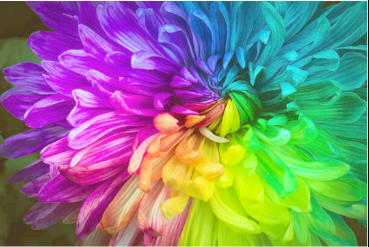
\includegraphics[width=9cm]{../Image_fonctions/Multicolor/EgalisationColor.PNG}
\end{center}
\begin{center} 
    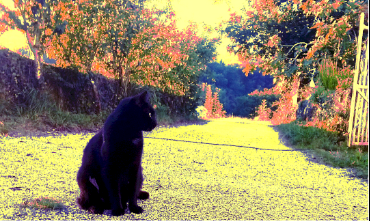
\includegraphics[width=9cm]{../Image_fonctions/Cat/EgalisationColor.PNG}
    
    (Image prise sur l'émulateur)
    
    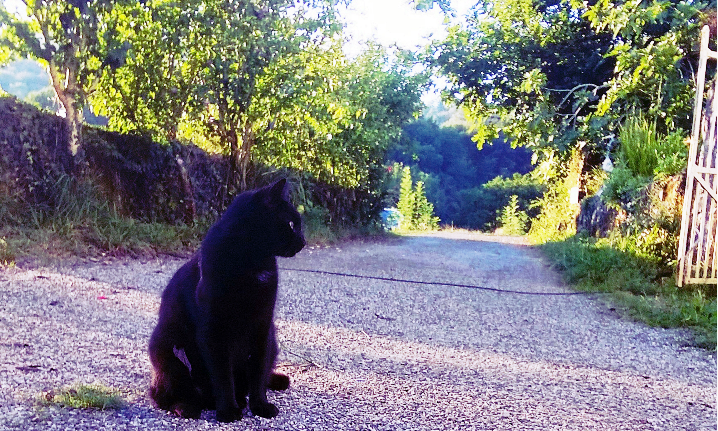
\includegraphics[width=9cm]{../Image_fonctions/Cat/EgalisationColor2.PNG}
    
    (Image prise sur le Sony)
\end{center}

\begin{center}
\medbreak
Test de performance de la fonction sur une image en couleur en microsecondes
\bigbreak
   \begin{tabular}{ | l | c | }
     \hline
     Image & Temps \\
     \hline
     Multicolor & 160 739 \\
     \hline
     Cat & 1 763 489 \\
     \hline
   \end{tabular}
 \end{center}
\bigbreak

\textbf{Remarques}
On remarque que les couleurs ne sont plus du tout fidèles à l'image de base (très visible sur l'image "multicolor").

\newpage
\subsection{TD 4 RenderScript}

% --- Gris RS --- %
\subsubsection{Griser l'image}

Cette fonction passe une image RGB en teintes de gris en utilisant le RenderScript.

\begin{center} 
    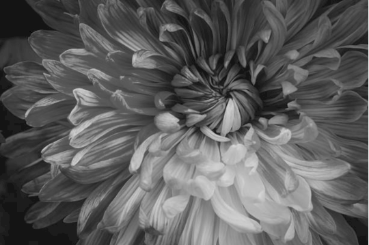
\includegraphics[width=9cm]{../Image_fonctions/Multicolor/GrayRS.PNG}
\end{center}
\begin{center} 
    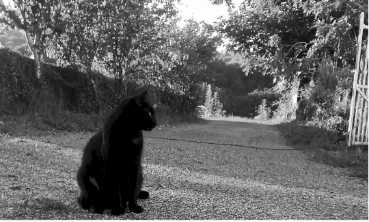
\includegraphics[width=9cm]{../Image_fonctions/Cat/GrayRS.PNG}
\end{center}

\begin{center}
\medbreak
Test de performance de la fonction lors du premier appel en microsecondes
\bigbreak
   \begin{tabular}{ | l | c | }
     \hline
     Image & Temps \\
     \hline
     Multicolor & 68 523 \\
     \hline
     Cat & 267 884 \\
     \hline
   \end{tabular}
 \end{center}
\bigbreak

\begin{center}
\medbreak
Test de performance de la fonction lors du second appel en microsecondes
\bigbreak
   \begin{tabular}{ | l | c | }
     \hline
     Image & Temps \\
     \hline
     Multicolor & 17 893 \\
     \hline
     Cat & 76 330 \\
     \hline
   \end{tabular}
 \end{center}
\bigbreak

% --- Negatif RS --- %
\subsubsection{Négatif}

Cette fonction passe une image RGB en négatif en utilisant le RenderScript.

\begin{center} 
    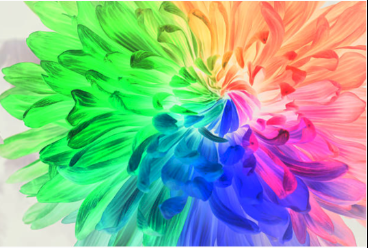
\includegraphics[width=9cm]{../Image_fonctions/Multicolor/NegativeRS.PNG}
\end{center}
\begin{center} 
    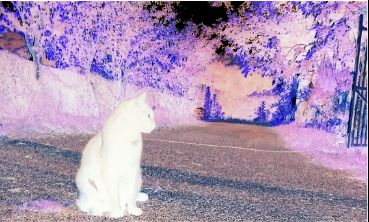
\includegraphics[width=9cm]{../Image_fonctions/Cat/NegativeRS.PNG}
\end{center}
\begin{center} 
    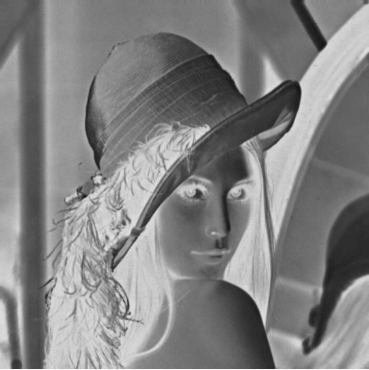
\includegraphics[width=9cm]{../Image_fonctions/Lenna/NegativeRS.PNG}
\end{center}

\begin{center}
\medbreak
Test de performance de la fonction lors du premier appel en microsecondes
\bigbreak
   \begin{tabular}{ | l | c | }
     \hline
     Image & Temps \\
     \hline
     Multicolor & 68 498 \\
     \hline
     Cat & 129 600 \\
     \hline
     Girl & 87 319 \\
     \hline
   \end{tabular}
 \end{center}
\bigbreak

\begin{center}
\medbreak
Test de performance de la fonction lors du second appel en microsecondes
\bigbreak
   \begin{tabular}{ | l | c | }
     \hline
     Image & Temps \\
     \hline
     Multicolor & 26 536 \\
     \hline
     Cat & 54 903 \\
     \hline
     Girl & 29 314 \\
     \hline
   \end{tabular}
 \end{center}
\bigbreak

% --- Autres --- %
\subsubsection{Autre tests}

J'ai pu coder les fonctions HSVtoRGB et RGBtoHSV afin de les implémentées dans les fonctions qui en ont besoin. Or cela me donne une image noire. J'ai aussi pu essayer le set d'une variable renderscript.

\newpage
% ------------ Convolution ----------- %
\subsection{TD 5/6 Convolution}

A partir du moment où l'utilisateur décide d'appliquer un filtre, l'image sera automatiquement en niveau de gris.

% --- Moyenneur --- %
\subsubsection{Moyenneur}

Cette fonction permet d'appliquer le filtre Moyenneur sur l'image courante. La fonction a été écrite de sorte qu'on puisse appliquer n'importe quelle taille de filtre (tant que cela forme un carré).

% 3x3 %
\textbf{-> 3x3}
Cette fonction applique un filtre 3x3 Moyenneur sur l'image en teintes de gris.

\begin{center} 
    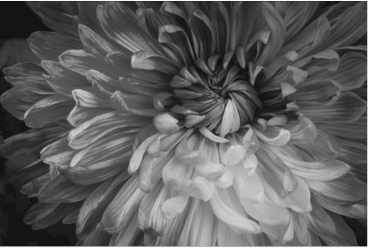
\includegraphics[width=9cm]{../Image_fonctions/Multicolor/Average3.PNG}
\end{center}
\begin{center} 
    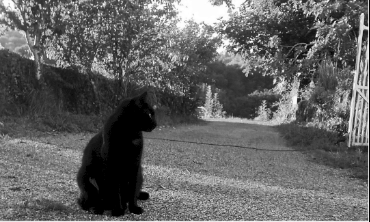
\includegraphics[width=9cm]{../Image_fonctions/Cat/Average3.PNG}
\end{center}
\begin{center} 
    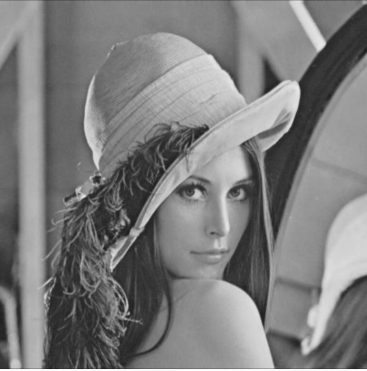
\includegraphics[width=9cm]{../Image_fonctions/Lenna/Average3.PNG}
\end{center}

\begin{center}
\medbreak
Test de performance de la fonction sur un filtre 3x3 en microsecondes
\bigbreak
   \begin{tabular}{ | l | c | }
     \hline
     Image & Temps \\
     \hline
     Multicolor & 1 266 906 \\
     \hline
     Cat & 6 150 486 \\
     \hline
     Girl & 1 316 911 \\
     \hline
   \end{tabular}
 \end{center}
\bigbreak

% 7x7 %
\textbf{-> 7x7}
Cette fonction applique un filtre 7x7 Moyenneur sur l'image en teintes de gris.

\begin{center} 
    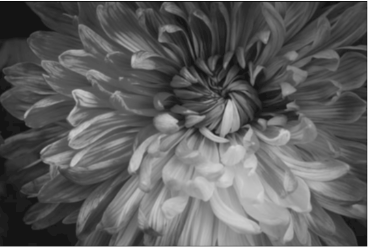
\includegraphics[width=9cm]{../Image_fonctions/Multicolor/Average7.PNG}
\end{center}
\begin{center} 
    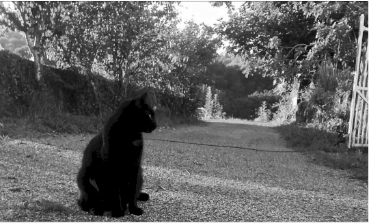
\includegraphics[width=9cm]{../Image_fonctions/Cat/Average7.PNG}
\end{center}
\begin{center} 
    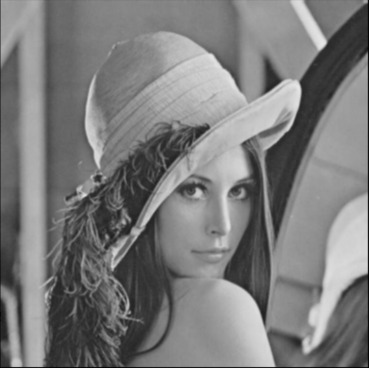
\includegraphics[width=9cm]{../Image_fonctions/Lenna/Average7.PNG}
\end{center}

\begin{center}
\medbreak
Test de performance de la fonction sur un filtre 7x7 en microsecondes
\bigbreak
   \begin{tabular}{ | l | c | }
     \hline
     Image & Temps \\
     \hline
     Multicolor & 3 807 841 \\
     \hline
     Cat & 27 989 316 \\
     \hline
     Girl & 4 098 690 \\
     \hline
   \end{tabular}
 \end{center}
\bigbreak

% 15x15 %
\textbf{-> 15x15}
Cette fonction applique un filtre 15x15 Moyenneur sur l'image en teintes de gris.

\begin{center} 
    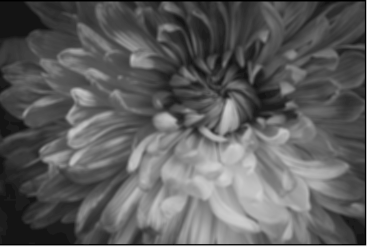
\includegraphics[width=9cm]{../Image_fonctions/Multicolor/Average15.PNG}
\end{center}
\begin{center} 
    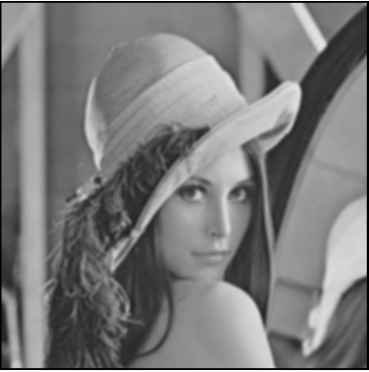
\includegraphics[width=9cm]{../Image_fonctions/Lenna/Average15.PNG}
\end{center}

\begin{center}
\medbreak
Test de performance de la fonction sur un filtre 15x15 en microsecondes
\bigbreak
   \begin{tabular}{ | l | c | }
     \hline
     Image & Temps \\
     \hline
     Multicolor & 16 017 509 \\
     \hline
     Cat & > 1min \\
     \hline
     Girl & 17 516 155 \\
     \hline
   \end{tabular}
 \end{center}
\bigbreak

% --- Gaussien --- %
\subsubsection{Gaussien}

Cette fonction permet d'appliquer le filtre Gaussien de taille 5x5 sur l'image courante.
\begin{center} 
    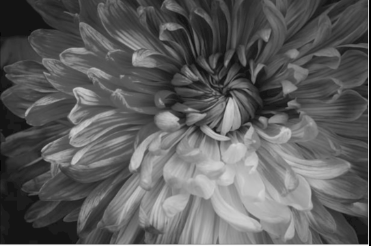
\includegraphics[width=9cm]{../Image_fonctions/Multicolor/Gaussien.PNG}
\end{center}
\begin{center} 
    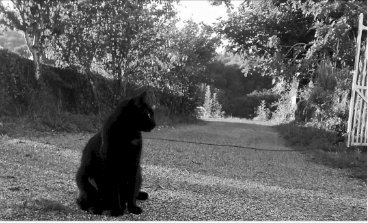
\includegraphics[width=9cm]{../Image_fonctions/Cat/Gaussien.PNG}
\end{center}
\begin{center} 
    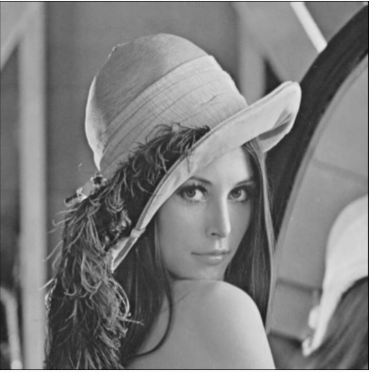
\includegraphics[width=9cm]{../Image_fonctions/Lenna/Gaussien.PNG}
\end{center}

\begin{center}
\medbreak
Test de performance de la fonction sur un filtre 15x15 en microsecondes
\bigbreak
   \begin{tabular}{ | l | c | }
     \hline
     Image & Temps \\
     \hline
     Multicolor & 2 988 799 \\
     \hline
     Cat & 20 197 782 \\
     \hline
     Girl & 2 227 218 \\
     \hline
   \end{tabular}
 \end{center}
\bigbreak

\subsubsection{Prewitt}

Cette fonction permet d'appliquer le filtre utilisant l'opérateur de Prewitt sur l'image courante.

\bigbreak
% Horizontal %
\textbf{-> Horizontal}

Cette fonction applique le filtre traitant seulement les contours horizontaux sur l'image en teintes de gris.

\begin{center} 
    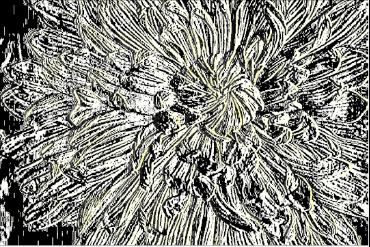
\includegraphics[width=9cm]{../Image_fonctions/Multicolor/PrewittH.PNG}
\end{center}
\begin{center} 
    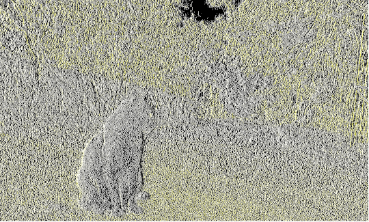
\includegraphics[width=9cm]{../Image_fonctions/Cat/PrewittH.PNG}
\end{center}
\begin{center} 
    \includegraphics[width=9cm]{../Image_fonctions/Lenna/PrewittH.PNG}
\end{center}

\begin{center}
\medbreak
Test de performance
 de la fonction en microsecondes
\bigbreak
   \begin{tabular}{ | l | c | }
     \hline
     Image & Temps \\
     \hline
     Multicolor & 1 203 671 \\
     \hline
     Cat & 6 292 324 \\
     \hline
     Girl & 916 858 \\
     \hline
   \end{tabular}
 \end{center}
\bigbreak

% Vertical %
\textbf{-> Vertical}

Cette fonction applique le filtre traitant seulement les contours verticaux sur l'image en teintes de gris.

\begin{center} 
    \includegraphics[width=9cm]{../Image_fonctions/Multicolor/PrewittV.PNG}
\end{center}
\begin{center} 
    \includegraphics[width=9cm]{../Image_fonctions/Cat/PrewittV.PNG}
\end{center}
\begin{center} 
    \includegraphics[width=9cm]{../Image_fonctions/Lenna/PrewittV.PNG}
\end{center}

\begin{center}
\medbreak
Test de performance de la fonction en microsecondes
\bigbreak
   \begin{tabular}{ | l | c | }
     \hline
     Image & Temps \\
     \hline
     Multicolor & 889 837 \\
     \hline
     Cat & 6 271 317 \\
     \hline
     Girl & 932 132 \\
     \hline
   \end{tabular}
 \end{center}
\bigbreak

% Tout %
\textbf{-> Horizontal et Verticaux}

Cette fonction applique les filtres traitant les contours horizontaux et verticaux sur l'image en teintes de gris.

\begin{center} 
    \includegraphics[width=9cm]{../Image_fonctions/Multicolor/Prewitt.PNG}
\end{center}
\begin{center} 
    \includegraphics[width=9cm]{../Image_fonctions/Cat/Prewitt.PNG}
\end{center}
\begin{center} 
    \includegraphics[width=9cm]{../Image_fonctions/Lenna/Prewitt.PNG}
\end{center}

\begin{center}
\medbreak
Test de performance de la fonction en microsecondes
\bigbreak
   \begin{tabular}{ | l | c | }
     \hline
     Image & Temps \\
     \hline
     Multicolor & 1 752 603 \\
     \hline
     Cat & 12 290 650 \\
     \hline
     Girl & 1 857 418 \\
     \hline
   \end{tabular}
 \end{center}
\bigbreak

% --- Sobel --- %
\subsubsection{Sobel}
Cette fonction permet d'appliquer le filtre utilisant l'opérateur de Sobel sur l'image courante.

\bigbreak
% Horizontal %
\textbf{-> Horizontal}

Cette fonction applique le filtre traitant seulement les contours horizontaux sur l'image en teintes de gris.

\begin{center} 
    \includegraphics[width=9cm]{../Image_fonctions/Multicolor/SobelH.PNG}
\end{center}
\begin{center} 
    \includegraphics[width=9cm]{../Image_fonctions/Cat/SobelH.PNG}
\end{center}
\begin{center} 
    \includegraphics[width=9cm]{../Image_fonctions/Lenna/SobelH.PNG}
\end{center}

\begin{center}
\medbreak
Test de performance de la fonction en microsecondes
\bigbreak
   \begin{tabular}{ | l | c | }
     \hline
     Image & Temps \\
     \hline
     Multicolor & 872 877 \\
     \hline
     Cat & 6 141 323 \\
     \hline
     Girl & 875 730 \\
     \hline
   \end{tabular}
 \end{center}
\bigbreak

% Vertical %
\textbf{-> Vertical}

Cette fonction applique le filtre traitant seulement les contours verticaux sur l'image en teintes de gris.

\begin{center} 
    \includegraphics[width=9cm]{../Image_fonctions/Multicolor/SobelV.PNG}
\end{center}
\begin{center} 
    \includegraphics[width=9cm]{../Image_fonctions/Cat/SobelV.PNG}
\end{center}
\begin{center} 
    \includegraphics[width=9cm]{../Image_fonctions/Lenna/SobelV.PNG}
\end{center}

\begin{center}
\medbreak
Test de performance de la fonction en microsecondes
\bigbreak
   \begin{tabular}{ | l | c | }
     \hline
     Image & Temps \\
     \hline
     Multicolor & 874 104 \\
     \hline
     Cat & 6 131 670 \\
     \hline
     Girl & 949 709 \\
     \hline
   \end{tabular}
 \end{center}
\bigbreak

% Tout %
\textbf{-> Horizontal et Verticaux}

Cette fonction applique les filtres traitant les contours horizontaux et verticaux sur l'image en teintes de gris.

\begin{center} 
    \includegraphics[width=9cm]{../Image_fonctions/Multicolor/Sobel.PNG}
\end{center}
\begin{center} 
    \includegraphics[width=9cm]{../Image_fonctions/Cat/Sobel.PNG}
\end{center}
\begin{center} 
    \includegraphics[width=9cm]{../Image_fonctions/Lenna/Sobel.PNG}
\end{center}

\begin{center}
\medbreak
Test de performance de la fonction en microsecondes
\bigbreak
   \begin{tabular}{ | l | c | }
     \hline
     Image & Temps \\
     \hline
     Multicolor & 1 730 116 \\
     \hline
     Cat & 12 393 357 \\
     \hline
     Girl & 1 855 651 \\
     \hline
   \end{tabular}
 \end{center}
\bigbreak

% --- Laplacien --- %
\subsubsection{Laplacien}

Cette fonction permet d'appliquer le filtre utilisant l'opérateur de Laplacien sur l'image courante.

% 4cx %
\textbf{4 cx}

Cette fonction applique le filtre 4 sur l'image courante.

\begin{center} 
    \includegraphics[width=9cm]{../Image_fonctions/Multicolor/Laplacien4.PNG}
\end{center}
\begin{center} 
    \includegraphics[width=9cm]{../Image_fonctions/Cat/Laplacien4.PNG}
\end{center}
\begin{center} 
    \includegraphics[width=9cm]{../Image_fonctions/Lenna/Laplacien4.PNG}
\end{center}

\begin{center}
\medbreak
Test de performance de la fonction en microsecondes
\bigbreak
   \begin{tabular}{ | l | c | }
     \hline
     Image & Temps \\
     \hline
     Multicolor & 881 344 \\
     \hline
     Cat & 6 121 870 \\
     \hline
     Girl & 927 105 \\
     \hline
   \end{tabular}
 \end{center}
\bigbreak

% 8 cx %
\textbf{-> 8 cx}

Cette fonction applique le filtre 8 sur l'image courante.

\begin{center} 
    \includegraphics[width=9cm]{../Image_fonctions/Multicolor/Laplacien8.PNG}
\end{center}
\begin{center} 
    \includegraphics[width=9cm]{../Image_fonctions/Cat/Laplacien8.PNG}
\end{center}
\begin{center} 
    \includegraphics[width=9cm]{../Image_fonctions/Lenna/Laplacien8.PNG}
\end{center}

\begin{center}
\medbreak
Test de performance de la fonction en microsecondes
\bigbreak
   \begin{tabular}{ | l | c | }
     \hline
     Image & Temps \\
     \hline
     Multicolor & 859 444 \\
     \hline
     Cat & 9 132 395 \\
     \hline
     Girl & 927 616 \\
     \hline
   \end{tabular}
 \end{center}

\newpage
% ----------- Autre ----------- %
\subsection{Autre}
\subsubsection{Negatif}

Cette fonction passe une image RGB en négatif.

\begin{center} 
    \includegraphics[width=9cm]{../Image_fonctions/Multicolor/Negative.PNG}
\end{center}
\begin{center} 
    \includegraphics[width=9cm]{../Image_fonctions/Cat/Negative.PNG}
\end{center}
\begin{center} 
    \includegraphics[width=9cm]{../Image_fonctions/Lenna/Negative.PNG}
\end{center}

\begin{center}
\medbreak
Test de performance de la fonction en microsecondes
\bigbreak
   \begin{tabular}{ | l | c | }
     \hline
     Image & Temps \\
     \hline
     Multicolor & 72 136 \\
     \hline
     Cat & 379 778 \\
     \hline
     Girl & 84 847 \\
     \hline
   \end{tabular}
 \end{center}
\bigbreak

% --- Saturation --- %
\subsubsection{Saturation}

Cette fonction permet de modifier la saturation (par tranche de +- 10 \%) de l'image courante.

% + 10 %
\textbf{+ 10 \%}
Cette fonction permet d'ajouter 10 \% à la saturation de l'image

\begin{center} 
    \includegraphics[width=9cm]{../Image_fonctions/Multicolor/Saturation+1.PNG}
\end{center}
\begin{center} 
    \includegraphics[width=9cm]{../Image_fonctions/Cat/Saturation+1.PNG}
\end{center}
\begin{center} 
    \includegraphics[width=9cm]{../Image_fonctions/Lenna/Saturation+1.PNG}
\end{center}

\begin{center}
\medbreak
Test de performance de la fonction en microsecondes
\bigbreak
   \begin{tabular}{ | l | c | }
     \hline
     Image & Temps \\
     \hline
     Multicolor & 758 694 \\
     \hline
     Cat & 5 515 344 \\
     \hline
     Girl & 790 574 \\
     \hline
   \end{tabular}
 \end{center}
\bigbreak

% - 10 %
\textbf{- 10 \%}
Cette fonction permet d'enlever 10 \% à la saturation de l'image

\begin{center} 
    \includegraphics[width=9cm]{../Image_fonctions/Multicolor/Saturation-1.PNG}
\end{center}
\begin{center} 
    \includegraphics[width=9cm]{../Image_fonctions/Cat/Saturation-1.PNG}
\end{center}
\begin{center} 
    \includegraphics[width=9cm]{../Image_fonctions/Lenna/Saturation-1.PNG}
\end{center}

\begin{center}
\medbreak
Test de performance de la fonction en microsecondes
\bigbreak
   \begin{tabular}{ | l | c | }
     \hline
     Image & Temps \\
     \hline
     Multicolor & 710 899 \\
     \hline
     Cat & 5 315 295 \\
     \hline
     Girl & 726 349 \\
     \hline
   \end{tabular}
 \end{center}
\bigbreak

% --- Luminosite --- %
\subsubsection{Luminosité}

Cette fonction permet de modifier la luminosité (par tranche de +- 10 \%) de l'image courante.

% + 10 %
\textbf{+ 10 \%}
Cette fonction permet d'ajouter 10 \% à la luminosité de l'image

\begin{center} 
    \includegraphics[width=9cm]{../Image_fonctions/Multicolor/Brightness+1.PNG}
\end{center}
\begin{center} 
    \includegraphics[width=9cm]{../Image_fonctions/Cat/Brightness+1.PNG}
\end{center}
\begin{center} 
    \includegraphics[width=9cm]{../Image_fonctions/Lenna/Brightness+1.PNG}
\end{center}

\begin{center}
\medbreak
Test de performance de la fonction en microsecondes
\bigbreak
   \begin{tabular}{ | l | c | }
     \hline
     Image & Temps \\
     \hline
     Multicolor & 755 021 \\
     \hline
     Cat & 5 502 287 \\
     \hline
     Girl & 775 903 \\
     \hline
   \end{tabular}
 \end{center}
\bigbreak

% - 10 %
\textbf{- 10 \%}
Cette fonction permet d'enlever 10 \% à la luminosité de l'image

\begin{center} 
    \includegraphics[width=9cm]{../Image_fonctions/Multicolor/Brightness-1.PNG}
\end{center}
\begin{center} 
    \includegraphics[width=9cm]{../Image_fonctions/Cat/Brightness-1.PNG}
\end{center}
\begin{center} 
    \includegraphics[width=9cm]{../Image_fonctions/Lenna/Brightness-1.PNG}
\end{center}

\begin{center}
\medbreak
Test de performance de la fonction en microsecondes
\bigbreak
   \begin{tabular}{ | l | c | }
     \hline
     Image & Temps \\
     \hline
     Multicolor & 749 832 \\
     \hline
     Cat & 5 211 125 \\
     \hline
     Girl & 737 299 \\
     \hline
   \end{tabular}
 \end{center}

\newpage
% ---------------- Bug ---------------- %
\section{Bugs}

% --- Interface --- %
\subsection{Interface}
\begin{itemize}
   
 \item Si on verrouille l'application et qu'on retourne dessus, on peut voir que la barre fixe revient, ce sera donc un problème à régler. 
    \item L'utilisation du menu déroulant pour les images remet aussi automatiquement la barre de navigation virtuelle fixe.
\end{itemize}

% --- Fonctions --- %
\subsection{Fonctions}
\begin{itemize}
    \item On peut remarquer des teintes jaunes apparaissant sur l'émulateur à l'égalisation de l'histogramme d'une image. Chose n'apparaissant pas sur le téléphone.
    \item Les fonctions HSVtoRGB et inversement ne fonctionnent pas en RenderScript, bloquant fortement l'écriture d'autres fonctions.
    \item On peut voir de l'apparition de jaune lors de l'application des filtres de Prewitt et de Sobel.
    \item Présence de "bruit" sur l'application du filtre de Laplacien. On peut voir aussi l'apparition d'une teinte jaune.
    \item En appliquant l'augmentation de la saturation sur une image en teintes de gris (ici "girl"), on peut voir l'apparition d'une teinte rosée.
\end{itemize}

\medbreak
Je pense que mes fonctions HSVtoRGB et RGBtoHSV modifies légèrement la teinte de mon image. Mais il y a des images qui sont toujours en noir et blanc, même lors de l'appel de ces fonctions.

Pour l'apparition de la teinte jaune lors de l'application de certains filtres, ont remarque que seuls les filtres ayant des coefficients négatifs sont touchés par ce bug, ce sera donc a corriger.

% ---------------- Limites ---------------- %
\section{Limites}
\begin{itemize}
    \item Seulement deux fonctions RenderScript implémentées.
    \item Pour la sélection de couleur, l'utilisation de boutons n'est pas pratique, lors du choix de la saturation/luminosité. Je pense implémenter une SeekBar afin d'effectuer ces modifications.
\end{itemize}
\end{document}